The code resides in \filename{src/cuda/} and only minor changes have been made to the original MarDyn code. These changes will be described in detail later as well.

The \cuda{} code shifts the molecule interaction calculation to the GPU. It calculates the interactions between different molecules using different potential models as specified in the component description\TODO{reference to Mardyn docs}.
A \cuda{} application performs basically three steps:
\begin{compactenum}
\item upload data to the GPU
\item process data on the GPU
\item download results from the GPU
\end{compactenum} 
Different information has to be uploaded in MarDyn. Information about the different molecule types (\textbf{component descriptions}) has to be uploaded only once. The position and orientation of every molecule has to be uploaded for each time step. 
Later the calculated forces and torque have to be downloaded, as well as the calculated potential and virial statistics.

The Linked Cells-algorithm is used in MarDyn. The simulation space is divided into a grid of cells and the interaction between molecules of the same and of neighboring cells have to be calculated. The length of the cells is chosen equal to the cutoff radius of the potential functions to make sure that only interactions of direct neighbors have to be calculated.
This leads to a natural parallelization approach:
\begin{compactitem}
\item for \textbf{intra-cell molecule interactions} each thread can process the molecules of one cell, and
\item for \textbf{inter-cell molecule interactions} each thread can process a different pair of neighboring cells.
\end{compactitem}

\subsection{General Architecture}
The \cuda{} code is made up of different components. Each component has exactly one responsibility.
The intention is to make it clear where changes go and make it easier to navigate the code.

A \textbf{component} usually consists of CPU and \cuda{} code which interact in a certain way. For this there usually are \filename{component.cpp} and \filename{component.h} files, which contain the CPU-side code, and a \filename{component.cum} file, which contains the \cuda{} code. \filename{.cum} stands for \textbf{cu}da \textbf{m}odule.

Normally you pass parameters as kernel parameters to \cuda{}. Separation of responsibilities is the main goal of having different components. Thus passing all paramaters as kernel parameters is not a good approach. The CPU code of each component needs a way to interact with the \cuda{} code and the 'glue' code should be part of the components and not be kept somewhere else\footnote{the first implementation used kernel parameters and the parameter count quickly became unacceptable}.

The solution is simple: \cuda{} supports global variables and the CPU/\cuda{} interface in each component uses global variables to exchange data. Different namespaces can be used for each component to avoid name conflicts. See \autoref{fig:component_architecture}.

Moreover, instead of global memory variables constant memory variables could be used. Constant memory has its own on-chip cache, so this is desirable. Since only little data is stored in constant memory, cache misses are unlikely.

\begin{figure}
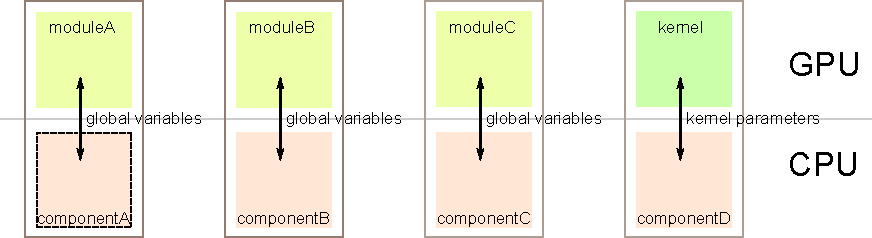
\includegraphics{figures/component_architecture.pdf}
\caption{components and \cuda{} modules}
\label{fig:component_architecture}
\end{figure}

\subsection{Component Overview}
Most components implement one of the two \lstinline!CUDAComponent! interfaces:
\begin{compactitem}
\item \lstinline!CUDAInteractionCalculationComponent! is used by components that perform data exchange operations at each time step, and
\item \lstinline!CUDAStaticDataComponent! is used by components that only need to upload data once.
\end{compactitem}

There are several components:
\begin{compactdesc}
\item[CellProcessor] contains logic to efficiently loop through the molecules of a single cell or a cell pair,
\item[ComponentDescriptor] manages the molecule component descriptions (eg the number of Lennard-Jones centers, their positions, etc),
\item[MoleculeInteraction] links all components together and calculates the forces,
\item[GlobalStats] keeps track of potential and virial statistics,
\item[MoleculePairHandler] calculates the interactions between two given molecules,
\item[MoleculeStorage] manages all per-molecule data like positions, forces and orientations,
\item[DomainTraverser] enumerates all cell pairs in a way that allows for maximum parallelization, and
\item[PotForce] calculates the force between Lennard-Jones centers, dipoles, etc.
\end{compactdesc}
See \autoref{fig:component_dep} for an overview how the different components interact with each other.

\begin{figure}
\centering
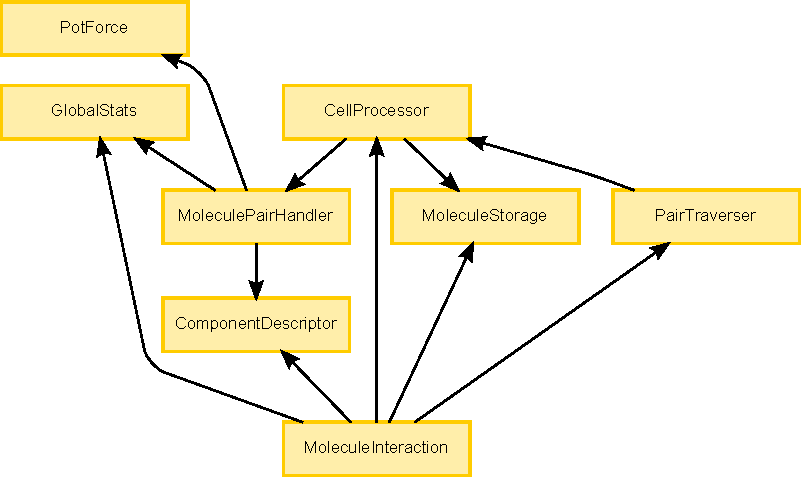
\includegraphics{figures/component_dependencies.pdf}
\caption{component dependencies (the arrows show which components each component uses, eg MoleculeInteraction uses GlobalStats)}
\label{fig:component_dep}
\end{figure}

There are additional \cuda{} modules that contain helper and utility functions.
All the \filename{.cum} files are included in \filename{kernel.cu}, which also contains the kernel entrance functions \lstinline!processCellPair! and \lstinline!processCell!, which are called by \textbf{MoleculeInteraction} to calculate the forces between all the molecules in a cell pair or in a single cell.

\subsection{\cuda{} Helper Classes and Functions}
\filename{helpers.cpp/h} contains C++ wrappers for \cuda{} functionality that is used.
It implements an internal DSL (see \cite{fowlerDSL} for a definition) to simplify working with the \cuda{} API. See \autoref{fig:helper_classes}.

\begin{figure}
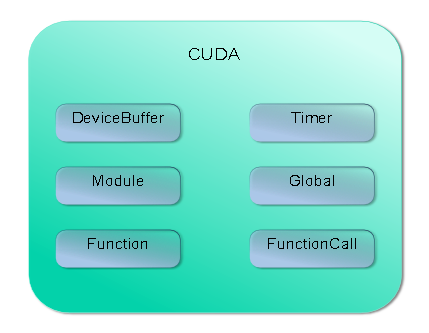
\includegraphics{figures/helpers_classes.pdf}
\centering
\caption{main \cuda{} helper classes}
\label{fig:helper_classes}
\end{figure}

\subsubsection{Device Buffers and Global Variables}
Managing device memory is done by creating instances of \lstinline!CUDA::DeviceBuffer<DataType>!. Methods are provided to resize the buffer and to copy data from and to the GPU.
Global variables are mapped to \lstinline!CUDA::Global<DataType>! objects. They provide a \lstinline!set! method that is specialized for pointer global variables to take \lstinline!CUDA::DeviceBuffer<DataType>! objects.
Example:
\begin{lstlisting}[label=cudamemoryhelpers,caption=\cuda{} helper classes for device memory and globals]
class GlobalStats : public CUDAInteractionCalculationComponent {
	CUDA::Global<CellStatsStorage *> _cellStats;
	CUDA::DeviceBuffer<CellStatsStorage> _cellStatsBuffer;
	
	GlobalStats( const CUDAComponent &component ) :
		_cellStats( _module.getGlobal<CellStatsStorage *>("cellStats") )
	/* ... */
	
		_cellStatsBuffer.resize( _linkedCells.getCells().size() );
		_cellStatsBuffer.zeroDevice();
		_cellStats.set( _cellStatsBuffer );		
	/* ... */		
};	
\end{lstlisting}

\subsubsection{Calling \cuda{} Functions}
The \lstinline!Function! class wraps \cuda{} functions. It has a \lstinline!call! method that returns a \lstinline!FunctionCall! object that can be used to specify the grid and block sizes and parameters before running the \cuda{} kernel by calling its \lstinline!execute! method.
Example:
\begin{lstlisting}[label=cudafunctionhelpers,caption=\cuda{} helper classes for function calls]
	CUDA::Function _convertQuaternionsToRotations;
/* ... */		
	MoleculeStorage( const CUDAComponent &component ) :
		_convertQuaternionsToRotations( _module.getFunction( "convertQuaternionsToRotations" ) )
/* ... */
		_convertQuaternionsToRotations.call().
			parameter(quaternionBuffer.devicePtr()).
			parameter(currentIndex).
			setBlockShape(MAX_BLOCK_SIZE, 1, 1).
			execute(currentIndex / MAX_BLOCK_SIZE + 1, 1);
\end{lstlisting}

\subsubsection{\filename{cutil\_double\_math.h}}
The \cuda{} SDK provides a helper file called \filename{cutil\_math.h} which adds overloaded operators and functions for most \cuda{} datatypes except \lstinline!double2!, \lstinline!double3! and \lstinline!double4!.
\filename{cutil\_double\_math.h} adds support for these datatypes.
This makes it possible to switch between single- and double-precision using a simple preprocessor \#define.

\subsubsection{Domain Traverser}
\begin{figure}
  \centering
  \subfloat[even start plane]{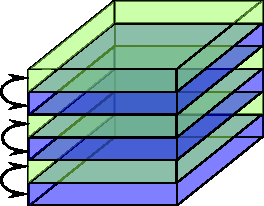
\includegraphics[width=0.5\textwidth]{figures/pairtraverser_even.pdf} }                
  \subfloat[odd start plane]{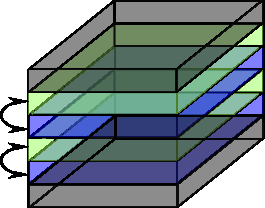
\includegraphics[width=0.5\textwidth]{figures/pairtraverser_odd.pdf} }
  \caption{schematic of the two steps the pair traverser performs}
\end{figure}
The simulation space is divided into a grid of cells. The domain traverser iterates over all neighbor pairings in the volume while maximizing parallelism. Each cell inside the volume has 26 neighbors. There are 13 directions because of symmetry: it doesn't matter if you calculate the interactions between cell A and B or cells B and A. This symmetry allows for a straight-forward parallelization.
I am going to introduce it using x-axis as interaction direction:
\begin{compactenum}
\item calculate the interactions between all cells $ \left ( 2*k, y, z \right ) $ and $ \left ( 2*k + 1, y, z \right ) $ in parallel (even case)
\item calculate the interactions between all cells $ \left ( 2*k + 1, y, z \right ) $ and $ \left ( 2*k + 2, y, z \right ) $ in parallel (odd case)
\end{compactenum}
It is easy to see that this covers all neighbor pairings along the x-axis.
The algorithm takes the even or odd layers parallel to the yz-plane and computes the interaction with the neighboring cells (along the x-axis).

All other directions can be treated like this. You only have to make sure that there are no out of boundary accesses.

The cells are flattened into a one-dimensional array and the CPU code calculates:
\begin{compactitem}
\item the index of the first cell (\lstinline!startIndex!)
\item the size of the two-dimensional grid that constitutes the parallel layers (\lstinline!dimension!)
\item offsets to move in x-, y- and z-direction in the one-dimensional cell array, whereas this constitutes a local coordinate system, such that the x- and y- span the two-dimensional grid and z- moves along the layers (\lstinline!gridOffsets!)
\item offset to get the neighbor cell for a cell along the currently used direction(\lstinline!neighborOffset!)
\end{compactitem}
With these parameters, the \lstinline!processCellPair! kernel can be launched in a grid of $ \text{dimension} \times \text{number of layers} $ thread blocks, that is one thread block per cell pair.

\subsection{Molecule Storage}
The molecule storage component manages everything related to molecule data. The molecules of all the cells are flattened into a one-dimensional array. For each cell the start index into this array is stored in a \lstinline!cellStartIndices! array. Since the start index of one cell is the end $ + 1 $ index of the cell before it, it is easy to extract all necessary information from this array.

Molecule data such as position, orientation, total force and torque, and molecule type, are stored non-interleaved into different buffers: \lstinline!moleculePositions!, \lstinline!moleculeRotations!, \lstinline!moleculeForces!, \lstinline!moleculeTorque! and \lstinline!moleculeComponentTypes!.

The molecule orientation is stored and uploaded as quaternions but converted to conventional $ 3 \times 3 $-matrices on the GPU.

The \cuda{} code wraps accesses to the data through a \lstinline!MoleculeStorage! class. The \lstinline!Molecule! class wraps accesses to it. This makes it possible to write the molecule interaction code without having to care for the actual implementation.

There is also a \lstinline!MoleculeLocalStorage<blockSize>! class. It provides a cache for frequently used molecules. Its objects are supposed to be instanciated as \lstinline!__shared__! objects and there are methods to load, merge and commit molecules from the cache to the regular storage.

\subsection{Component Descriptors}
Each molecule has a related \lstinline!moleculeComponentTypes! attribute, which specifies which component the molecule belongs to.

The component descriptor specifies common properties of molecules:
\begin{compactitem}
\item number of sites: Lennard-Jones centers, charges and dipoles
\item position of a site relative to the molecule centers
\item site-specific properties like $\epsilon$ and $\sigma$ parameters for Lennard-Jones centers or $\left  | \mu \right | $ for dipoles.
\end{compactitem}
The properties of the different sites are stored in fixed-size arrays.
Their sizes are set by the compile-time constants \lstinline!MAX_NUM_LJCENTERS!, \lstinline!MAX_NUM_CHARGES! and \lstinline!MAX_NUM_DIPOLES! respectively.
The number of supported components is set by the compile-time constant \lstinline!MAX_NUM_COMPONENTS!.

The mix coefficients $\xi$ and $\eta$ are stored in two 2D arrays.

\subsection{Global Statistics}
The potential and virial are calculated per cell on the GPU. For this the GPU code creates shared arrays for one potential and one virial value per thread in a threadblock, so the values can be updated by their threads without synchronization. The \lstinline!CellStatsCollector! class has a \lstinline!reduceAndStore! method which sum-reduces the two arrays into cell potential and cell virial values.

It does this by first summing all potentials inside a warp without any locking. Then it loops over all warps and reduces them sequentially.

The CPU code then reduces these per-cell values into per-domain values. Potentials and virials are calculated per molecule pair and added to the cells the molecules belong to. In the case of molecules from the same cell, the values are added to the same cell twice. Now the domain values, as sum of all cell values, count each potential and virial value twice, so the code halves the values.

There is also a difference compared to the regular MarDyn code: the force interaction code in MarDyn defines \lstinline!distanceAtoB! as \lstinline!positionA - positionB!, while the \cuda{} code defines it as \lstinline!positionB - positionA!, which makes more sense sementically. Because of this sign change, the calculated GPU virial has to be sign inverted, too, to match the CPU virial value.

\subsection{PotForce}
This component mostly mirrors the corresponding \filename{potforce.h} file in the CPU code except for sign changes as described in the previous paragraph. Only the dipole-dipole code has been refactored to use fewer operations.

\subsection{Molecule Pair Handler}
The molecule pair handler resolves the interactions of a molecule pair. All supported potential models are independent of the neighborhood of the two molecules, so only the two molecules are passed as paramaters.

First the pair handler tests whether the molecule centers are within the cutoff radius. Otherwise no interactions are calculated.

After that the molecule pair handler loads the component descriptors for each molecule and iterates through all sites as necessary to calculate the interactions. It also adds the calculated potential and virials to the global stats.

To calculate the interactions it needs to know the distance between the sites of the molecules. For this it transforms the relative position of each site as specified in the component descriptors using the \lstinline!moleculeRotations! matrices that have been created from the quaternions. Once all needed values have been determined, it uses the methods in the PotForce component to determine the actual forces and torque.

\subsection{Cell Processor}
The cell processor processes all molecules in the same cell (intra-cell) or between two cells (intra-cell).
The reference approach is to iterate through all molecule pairs in both cells and calculate the interactions between them:
\begin{figure}
  \centering
  \subfloat[first eight molecule interactions]{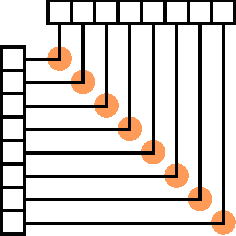
\includegraphics[width=0.3\textwidth]{figures/cellprocessor_first_iteration.pdf} }                
  \subfloat[all inter-cell interactions]{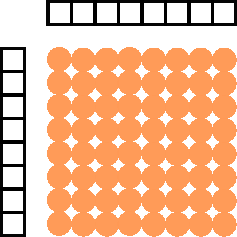
\includegraphics[width=0.3\textwidth]{figures/cellprocessor_all_iterations_inter_cell.pdf} }
  \subfloat[all intra-cell interactions]{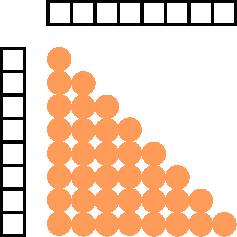
\includegraphics[width=0.3\textwidth]{figures/cellprocessor_all_iterations_intra_cell.pdf}}
  \caption{schematic of molecule interactions between two cells}
\end{figure}

\begin{lstlisting}[label=intercellreferenceloop,caption=reference inter-cell block processing]
__device__ void processCellPair( const int threadIndex, const CellInfo &cellA, const CellInfo &cellB ) {
	for( uint indexA = cellA.startIndex ; indexA < cellA.endIndex ; indexA++ ) {
		StorageMolecule moleculeA(indexA);

		for( uint indexB = cellB.startIndex ; indexB < cellB.endIndex ; indexB++ ) {
			StorageMolecule moleculeB(indexB);
			MoleculePairHandler::process( 0, moleculeA, moleculeB );
			moleculeB.store();
		}
		moleculeA.store();
	}
}
\end{lstlisting}
The intra-cell case is similar. The only difference is that only half of the interactions have to be calculated, because order\footnote{molecule A with molecule B is the same as molecule B with molecule A} does not matter:
\begin{lstlisting}[label=intracellreferenceloop,caption=reference intra-cell block processing]
__device__ void processCell( const int threadIndex, const CellInfo &cell ) {
	for( uint indexA = cell.startIndex ; indexA < cell.endIndex ; indexA++ ) {
		StorageMolecule moleculeA(indexA);

		for( uint indexB = cell.startIndex ; indexB < indexA; indexB++ ) {
			StorageMolecule moleculeB(indexB);
			MoleculePairHandler::process( 0, moleculeA, moleculeB );
			moleculeB.store();
		}
		moleculeA.store();
	}
}
\end{lstlisting}

\paragraph{Thread Block Cell Processor}
The main idea in the parallelized approach is to divide the cells into smaller blocks that can be kept in shared memory and process interactions inside between the different blocks. Parallelized matrix multiplication is based on the same idea. See \cite{cuda11progguide}.

Thus the cell processor divides the cells into blocks. Each block contains exactly one molecule for each thread in a thread block.
The code then iterates over all block pairs in both cells and calculates the interactions between molecules of the two blocks.
The inter-cell case is straight-forward:
\begin{lstlisting}[label=intercellloop,caption=inter-cell block processing (thread block cell processor)]
for( int blockIndexA = 0 ; blockIndexA < numBlocksA ; blockIndexA++ )
	for( int blockIndexB = 0 ; blockIndexB < numBlocksB ; blockIndexB++ )
		processBlock<BPT_UNRELATED>( /* ... */ );
\end{lstlisting}
For the intra-cell case only half of the block pairs have to be processed, because again it does not matter if block A with block B are processed of vice-versa:
\begin{lstlisting}[label=intracellloop,caption=intra-cell block processing (thread block cell processor)]
for( int blockIndexA = 0 ; blockIndexA < numBlocksA ; blockIndexA++ ) {
	processBlock<BPT_SAME_BLOCK>( /* ... */ );
	
	for( int blockIndexB = 0 ; blockIndexB < blockIndexA; blockIndexB++ )
		processBlock<BPT_UNRELATED>( /* ... */ );
}
\end{lstlisting}
Likewise, the calculation of interactions inside the same block (ie intra-block) have to be treated as special case.

Since there are as many threads as molecules in a block, each thread can be assigned a fixed molecule of block A (in the outer loop). This molecule can be stored in registers or in local memory.
The molecules of block B (of the inner loop) can be stored in shared memory, since they are only accessed by diffferent threads of the same thread block.

\begin{figure}
\centering
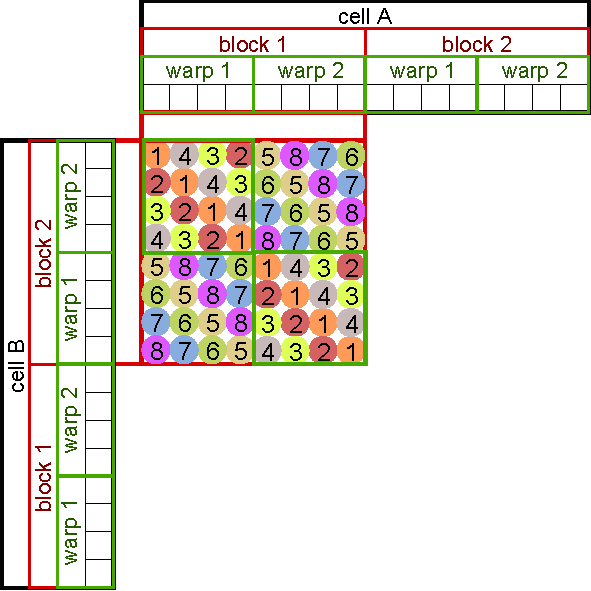
\includegraphics{figures/cellprocessor_block_iteration_1.pdf}
\caption{schematic of one block iteration (with a thread blocks of size 8 and warps of size 4, and all 8 parallel molecule pair iterations are shown for the block pair)}
\end{figure}

A straight-forward algorithm would simply loop over all molecules in block B and each thread would calculate the interactions of its fixed molecule from block A with one molecule from block B.
This is not the best solution however. Instead a block is divided into \textbf{warp blocks}. Each warp block contains 32 molecules (exactly the warp size).
The aim here is not to improve cache usage, but to require less explicit synchronization.
In the naive approach there would have to be a barrier after each interaction calculation to make sure that each thread is done with processing its molecule pair because another thread will access the molecule from block B in shared memory next.
Threads in the same warp are synchronized by design, because they are executed in lockstep, so processing  molecule interactions warp-block by warp-block improves parallelism.
Again there is a special case when interactions of molecules of the same warp-block are calculated.

\subsection{Warp Block Cell Processor}
Another cell processor was adedd, because the performance of the thread block cell processor, which we have just looked at, does not scale well for sparsely populated cells. 

The main problem is the sparse granularity of the thread block cell processor, which assigns the same amount of warps to each cell regardless of the number of molecules in it. The warp block cell processor fixes this.

It works by using a dynamic scheduler and it processes cells on warp level. This means that a cell or cell pair is not processed by exactly one thread block, but by a varying number of warps inside possibly different thread blocks.

One thread block is running on each SM. A thread block can ask for jobs which are assigned to its different warps. A short jobs queue is used for every warp. Each warp processes a warp block inside the cell. For cell pairs the warp block inside one cell stays fixed while it iterates over all molecules of the other cell.

To synchronize all thread blocks and warps a global mutex is used. Idle warps try to acquire the lock and get new jobs. Multiple warps of the same thread block are joined together to reduce the amount of locking needed.

Because every warp calculates interactions on its own, storing back potential and virial values requires a per-cell lock to avoid race conditions.

There are two different implementations for calculating interactions. The simpler one calculates all  interactions twice: between molecules in cells A and B and between molecules in cells B and A.
The molecules of cell A are assigned to different warps and each warp iterates over all molecules in cell B and calculates the interactions and only stores them back into the molecules of cell A.
When this is done, the cells are switched and now all interactions are calculated again and stored back into cell B.
This avoids the need for additional locks and synchronization.

\begin{lstlisting}[caption=inter-cell block processing (warp block cell processor)]
if( indexA >= warpBlockA.cell.endIndex ) {
	return;
}

StorageMolecule moleculeA;
moleculeA.init(indexA);

// now loop over all molecules in this cell
CellInfo cellB = warpBlockPairInfo.cellB;

for( int indexB = cellB.startIndex ; indexB < cellB.endIndex ; indexB++ ) {
	StorageMolecule moleculeB;
	moleculeB.init(indexB);

	MoleculePairHandler::process( getThreadIndex(), moleculeA, moleculeB );
}

moleculeA.store();
\end{lstlisting}

The other implementation only calculates all interactions once and writes them to molecules from both cells. However, it needs additional locking because multiple warps might attempt to write into cell B at the same time. It uses shared memory to cache several molecules and iterate over them before writing them back. This reduces the amount of locking needed.

\begin{lstlisting}[caption=inter-cell block processing with shared memory cache(warp block cell processor)]
StorageMolecule moleculeA;
moleculeA.init(indexA);

// now loop over all molecules in this cell
CellInfo cellB = warpBlockPairInfo.cellB;
for( int indexB = cellB.startIndex ; indexB < cellB.endIndex ; indexB += WARP_SIZE ) {
	const uint threadIndex = getThreadIndex();
	resultLocalStorage.reset( threadIndex );

	if( indexA < cellA.endIndex ) {
		for( int shift = 0 ; shift < WARP_SIZE ; shift++ ) {
			const uint shiftedWarpThreadIdx = (warpThreadIdx + shift) % WARP_SIZE;
			const uint moleculeIndex = indexB + shiftedWarpThreadIdx;

			ResultStorageMolecule moleculeB;
			moleculeB.init( moleculeIndex );

			if( indexB + shiftedWarpThreadIdx < cellB.endIndex ) {
				MoleculePairHandler::process( threadIndex, moleculeA, moleculeB );

				const int targetIndex = warpIdx * WARP_SIZE + shiftedWarpThreadIdx;
				moleculeB.store( targetIndex );
			}
		}
	}

	// store the processed molecules
	if( warpThreadIdx == 0 ) {
		cellLocks[cellIndexA].lock();
	}

	if( indexB + warpThreadIdx < cellB.endIndex ) {
		resultLocalStorage.commit( threadIndex, indexB + warpThreadIdx );
	}

	__threadfence();

	if( warpThreadIdx == 0 ) {
		cellLocks[cellIndexA].unlock();
	}
}

if( indexA < cellA.endIndex ) {
	moleculeA.store();
}
\end{lstlisting}

\subsection{MarDyn Integration}
The \cuda{} code is intergrated into MarDyn by the \lstinline!LinkedCellsCUDADecorator! class. It implements the \lstinline!ParticleContainer! interface and decorates an internal \lstinline!LinkedCells! object to calculate the molecule interactions using the GPU instead of the CPU.
The main assumption of the code is that the cut-off radius is less than or equal to the size of a cell, so that only interactions between molecules of the same cell or between direct neighbors have to be calculated.

There are only few changes to MarDyn's code. The \lstinline!MoleculeStorage! class is a friend of \lstinline!Molecule!, a \lstinline!setStats! method has been added to \lstinline!ParticlePairs2PotForceAdapter! and additional accessor methods were needed in \lstinline!LinkedCell!.

\subsection{Debug and Testing Code}
To verify that the \cuda{} implementation works correctly, there is code to run the CPU and \cuda{} interaction code in parallel and compare the calculated forces and torque.
This option can be enabled by uncommenting \lstinline!#define COMPARE_TO_CPU! in \filename{cuda/config.h}.

Likewise there is code to disable the fast cell processor and use the reference implementation which is not parallelized at all and simple iterates over all molecules in the cells.
It can be enabled by uncommenting \lstinline!#define REFERENCE_IMPLEMENTATION! in \filename{cude/config.h}.

To output the component descriptors as uploaded to the GPU, uncomment \lstinline!#define DEBUG_COMPONENT_DESCRIPTORS! and to verify that the quaternion to matrix conversion works properly uncomment \lstinline!#define TEST_QUATERNION_MATRIX_CONVERSION!.

\subsection{\filename{cuda/config.h}}
The config header allows you to customize and choose different code paths. It is possible to switch between single-precision and double-precision calculations on the GPU and to configure the number of supported component sites such as the number of Lennard-Jones centers or dipoles.
